\newpage
\section{Структура работы}
Для реализации нашего проекта мы решили воспользоваться возможностями языка JavaScript. Наш проект состоит из двух важных моментов, над которыми мы в основном работали по отдельности. Интерактивная модель мозга, отображающая основные структуры мозга и обучающий тест, позволяющий пользователю оценить пробелу в знании. 

\textbf{ Главная страница }


\begin{figure}[H]
	\center{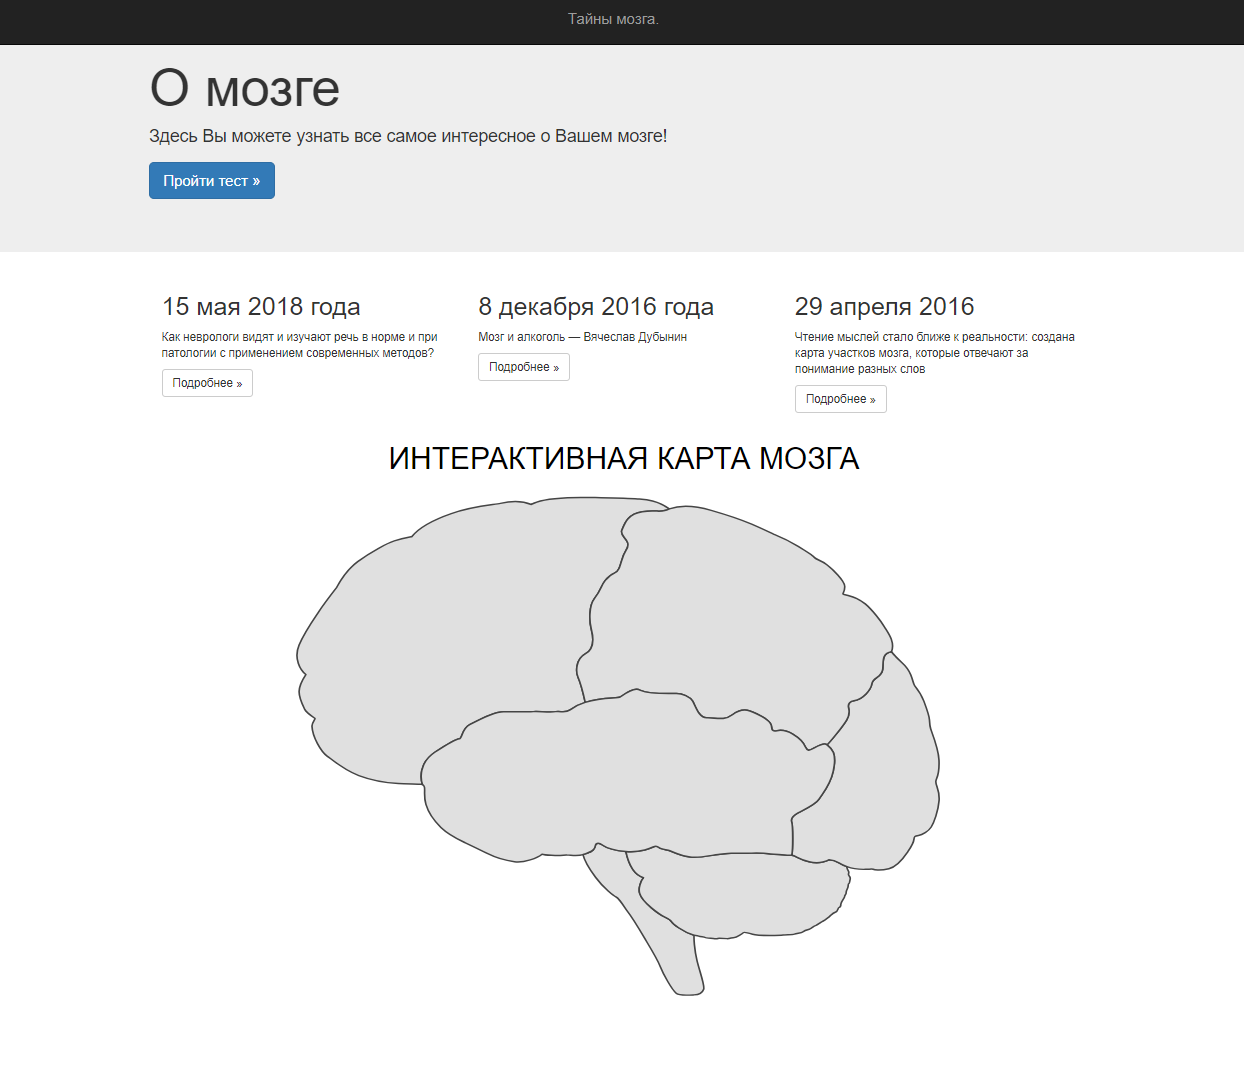
\includegraphics[width=1\linewidth]{8}}
	\caption{Главная страница ресурса}
	\label{ris:m}
\end{figure}


\subsection{Создание обучающего теста}
Созданием обучающего теста и сайта, на котором все расположено в основном занимался мой коллега, поэтому я не стану сильно распространяться, вы можете ознакомиться подробнее в его работе. 

Отмечу лишь несколько отличительных черт. Этот тест является не обычной проверкой знаний. Он носит образовательный характер из-за того что ответы даются пользователю сразу же после ответа и являются развернутыми ответами с примерами и доказательствами. За основу брались важные, на наш взгляд, заблуждения, связанные с работой мозга, о которых стоит знать правду.  




\subsection{Интерактивная карта мозга}
Изначальная задумка была, создать трехмерную интерактивную карту мозга, однако в последствии я пришел к выводу, что сделать это не представляется возможным в те сроки, что были отведены. Поэтому решили остановиться на 2д модели. Разумеется в качестве основы использовалось векторное изображение в формате SVG \footnote{Scalable Vector Graphics — масштабируемая векторная графика}, взятое из открытого источника. Векторное изображение позволяет масштабировать без потери качетсва, это то что нужно для наглядной демонстрации. Для построения карты мозга использовалась библиотека raphael, которая позволяет достаточно быстро и красиво отрисовать любую карту. Для обработки событий(интерактивности) использовалась библиотека jQuery. Карта выглядит следующим образом(рис.1). При наведении курсором мыши на область происходит её выделение. При нажатии появляется окошко, в котором представлена основная информация. Смотрите рис.2
\begin{figure}[h]
	\center{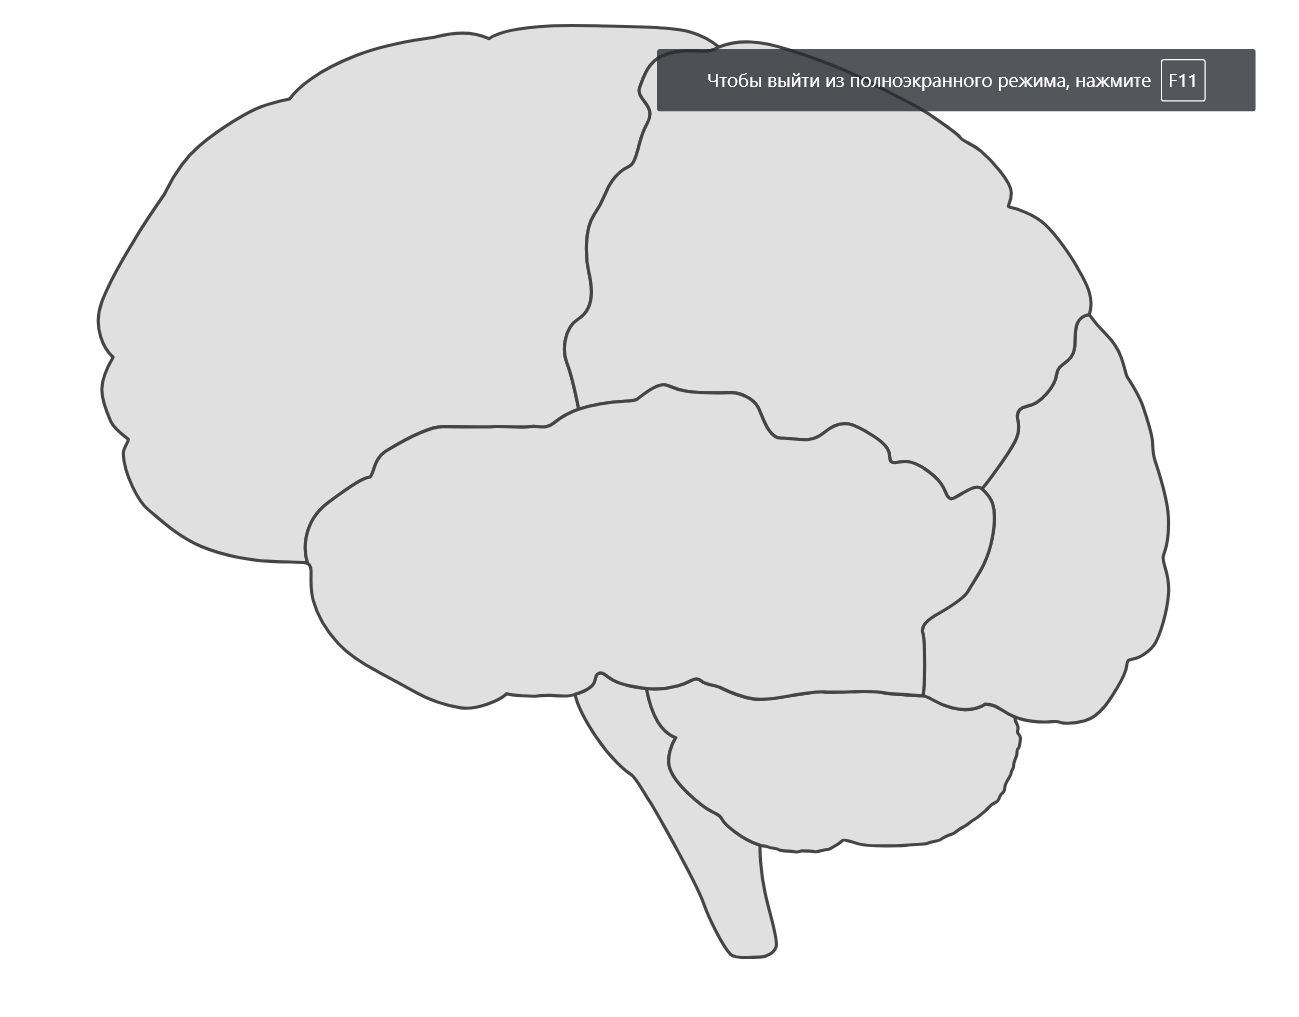
\includegraphics[width=0.8\linewidth]{4}}
	\caption{Карта мозга без взаимодействия}
	\label{fig:1}
\end{figure}
\begin{figure}[H]
	\center{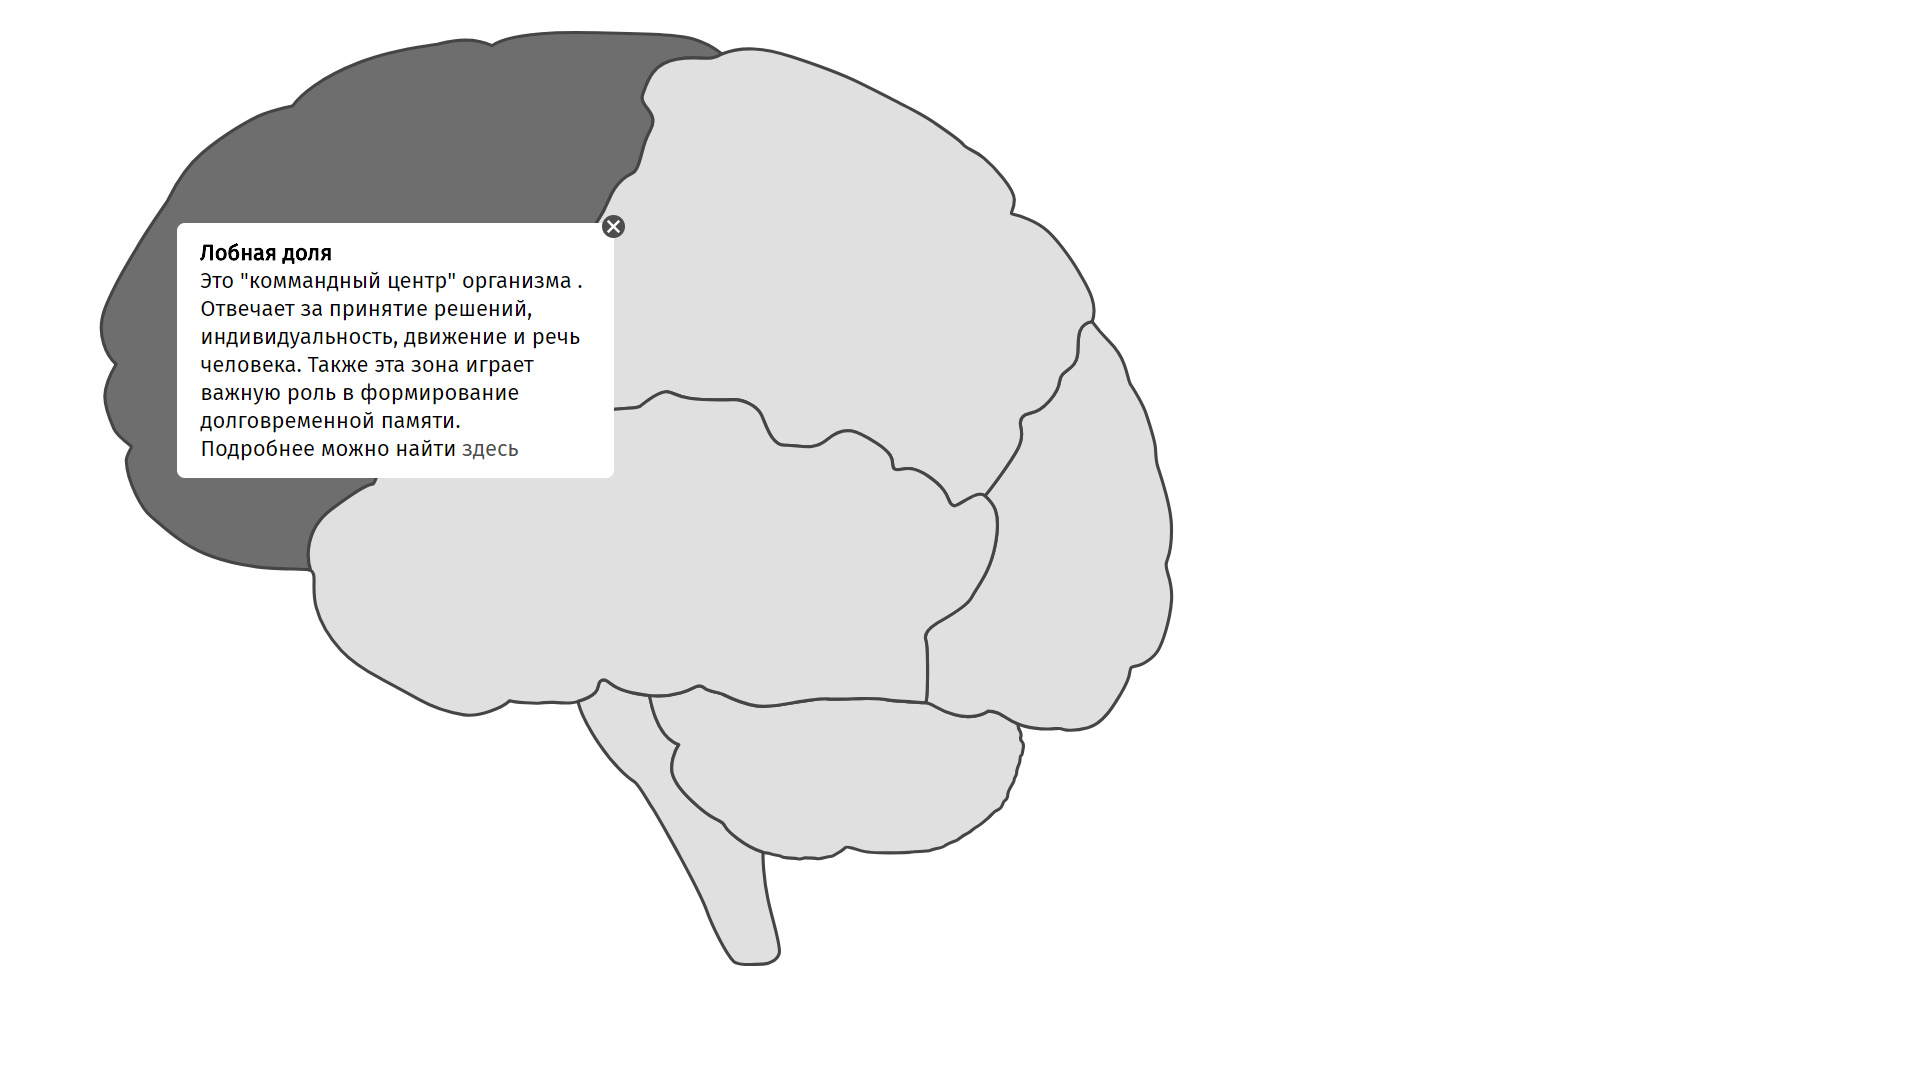
\includegraphics[width=0.8\linewidth]{2}}
	\caption{Карта мозга при нажатии курсора мыши}
	\label{fig:2}
\end{figure}

Теперь давайте поговорим более предметно, как происходит построение карты. Перво-наперво необходимо создать массив из различных зон, представленных в svg коде. Также каждому элементу массива присваивается информация об участке. Пример на рис. \ref{ris:mas}
\begin{figure}[h]
	\center{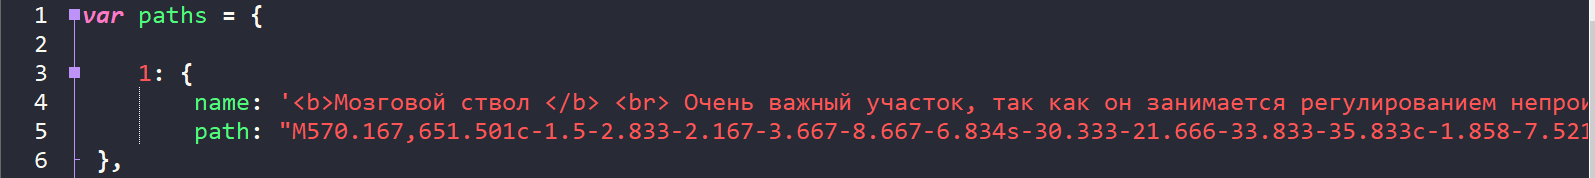
\includegraphics[width=1\linewidth]{5}}
	\caption{Элемент массива}
	\label{ris:mas}
\end{figure}

Далее происходит создание холста, определенного размера, на котором будет размещена наша карта, задаются специальные аттрибуты отрисовки(цвет заливки, цвет и ширина контура и размеры). 
После этого программа отрисовывает каждый контур с использованием заданных атрибутов, а также с помощью библиотеки jQuery взаимодействие. Вы можете видеть, что сначала прописывается действие при наведение курсора, а затем при нажатии. Также добавлена кнопка "закрыть", позволяющая скрыть окошко с информацией. Код представлен ниже, для того, чтобы сделать его более понятным написаны комментарии.
\begin{figure}[h]
	\center{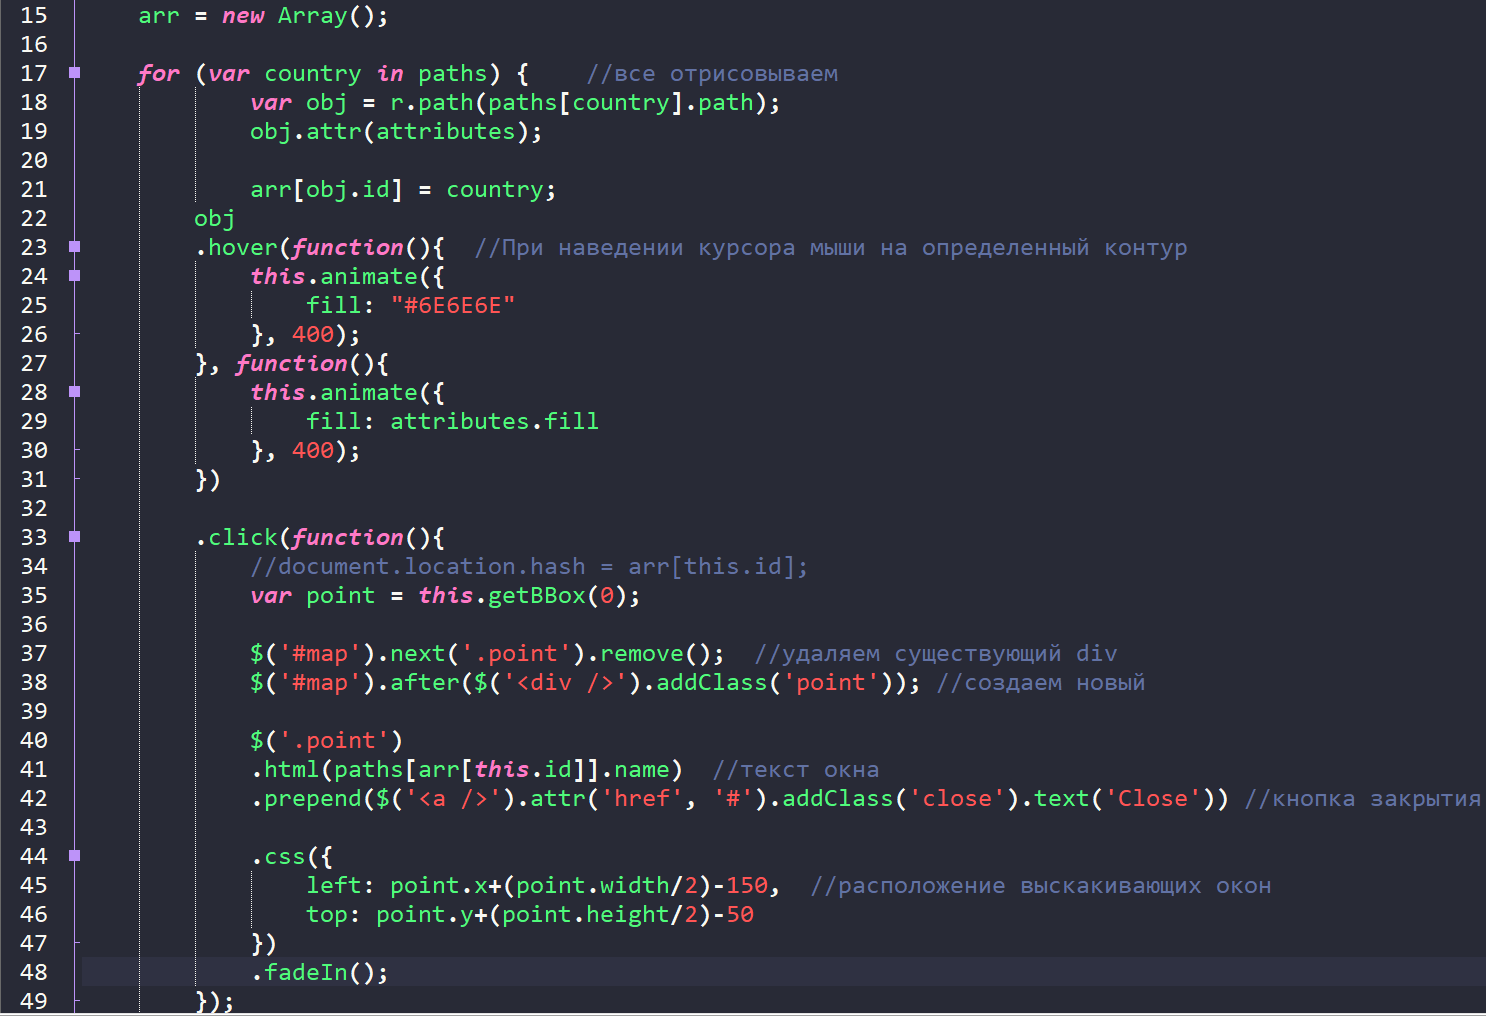
\includegraphics[width=1\linewidth]{6}}
	\caption{Отрисовка контуров, действия при наведении и при нажатии на контур}
	\label{ris:m}
\end{figure}

\begin{figure}[h]
	\center{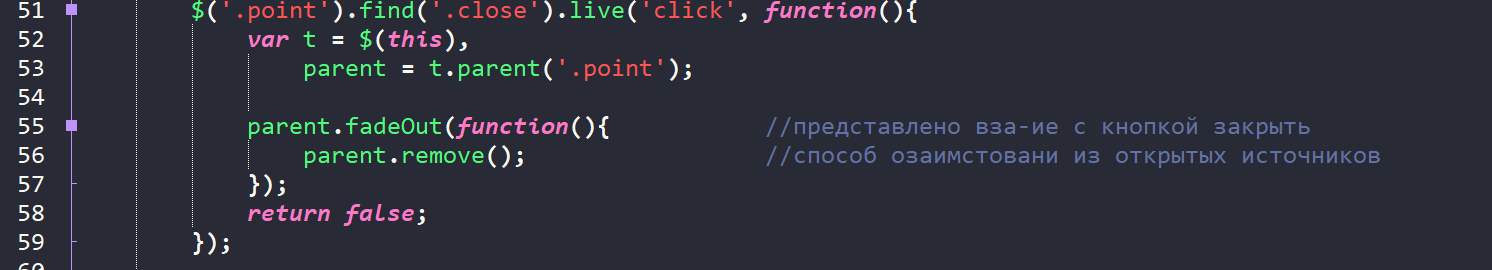
\includegraphics[width=1\linewidth]{7}}
	\caption{Работа кнопки закрыть}
	\label{ris:m}
\end{figure}



\section{Заключение}
В процессе выполнения работы, я познакомился со способами построения интерактивных карт, с возможностями библиотеки raphael и jQuery. Также я больше узнал о работе мозга, и о заблуждениях, о некоторых я даже не догадывался. Моим коллегой был составлен обучающий тест, а также сайт на котором всё располагается. Сервис получился довольно приятным в использовании. Мы очень надеемся на то, что проект принесет пользу для обычных пользователей и они смогут узнать что-то о самом сложном органе во вселенной. 